%%%%%%%%%%%%
%% This is the CWRU thesis template for PhD and Masters degree theses. The template file cwru_thesis.cls and this main.tex file follow the guidelines of the school of graduate studies found at https://case.edu/gradstudies/current-students/electronic-theses-and-dissertation-guidelines as of February 2023, with the inclusion of an additional List of Symbols if desired.
%%
%% This .tex file is for use with BibLaTeX.
%%
%% As of Spring 2023, the School of Graduate Studies requires some minimum accessibility requirements for all electronic theses. Accessibility is difficult to produce with LaTeX on the front end, but fortunately it is quite easy to meet the requirements on the back end using Adobe (not Adobe Reader). Simply download the PDF of your thesis and follow this guide: https://case.edu/gradstudies/sites/case.edu.gradstudies/files/2023-02/CWRU%20Thesis%20and%20Dissertation%20Accessiblity%20Guide_0.pdf
%%%%%%%%%%%%

\documentclass[12pt]{cwru_thesis}
\usepackage[hyphens]{url}
\usepackage{lipsum}
\usepackage{graphicx}
\usepackage{hyperref}
\hypersetup{colorlinks=true, linkcolor=black, filecolor=black, urlcolor=black, citecolor=black}
\urlstyle{same}
% \usepackage[acronym,toc]{glossaries}
\usepackage[intoc]{nomencl}
\renewcommand{\nomname}{List of Symbols}

\usepackage{mathptmx}
\usepackage[T1]{fontenc}
\usepackage[utf8]{inputenc}
\usepackage{amsfonts, amsmath, amsthm, amssymb}


\newcommand{\dif}{\mathrm{d}}
\newcommand{\Dif}{\mathrm{D}}
\renewcommand{\vec}[1]{\ensuremath{\underline{#1}}}
\newcommand{\grad}{\underline{\nabla}}
\newcommand{\curl}{\underline{\nabla} \times}
\newcommand{\lap}{\underline{\nabla}^2}
\renewcommand{\div}{\underline{\nabla} \cdot}
\newcommand{\paren}[1]{\left( {#1} \right)}
\newcommand{\norm}[1]{\lVert#1\rVert}

% Must use biblatex to produce the Published Contents and Contributions, per-chapter bibliography (if desired), etc.
\usepackage[
    backend=biber,natbib,style=numeric-comp,maxbibnames=99
]{biblatex}

% Name of your .bib file(s)
\addbibresource{example.bib}

% \makeglossaries
%%%%%%%%%%%%%%%%%%%%%%%%%%%%%%%%%%%%%%%%%%%%%%%%%%%%%%%%%%%%%%%%%%%%%%%%%%%%%%%%%%%%%%%
%Glossary entries


%Acronyms to include in the list of acronyms
% \newacronym{mda}{MDA}{Multipath Discovery Algorithm}
% \newacronym{mca}{MCA}{Multipath Classification Algorithm}

\begin{document}
\pagenumbering{roman}

% Do remember to remove the square brackets!
\title{Omar's Thesis} %Title of your thesis in title case
\author{Omar Loudghiri} %Your name

\degreeaward{Master's of Science in Computer Science}                 % Degree to be awarded
\department{Department of Computer Science and Data Science}
\university{Case Western Reserve University}    % Institution name  
\unilogo{cwru_logo.eps}                                 % Institution logo
\defendmonth{August, 2024}          % Graduation month and year
\defenddate{July 10th, 2024}          % Date of thesis defense

%Committee Member names. If you have a different number of committee members for your defense, you will need to edit lines 183-190 of cwru_thesis.cls accordingly.
\committeeChair{An Wang} %Committee Chair's name
\committeeOne{Mark Allman} %Committee member #1's name
\committeeTwo{Vincenzo Liberatore} %Committee member #2's name
\committeeThree{Mehmet Koyuturk} %Committee member #3's name

%%  If you'd like to add the CWRU logo from your title page, simply add the "[logo]" text to the maketitle command. Note that the School of Graduate Studies doesn't like this.
\maketitle

\begin{dedication} 	 
  TBD
\end{dedication}

\begin{KeepFromToc}
  \tableofcontents
\end{KeepFromToc}
\listoftables
\listoffigures



\begin{acknowledgements}
   TBD
\end{acknowledgements}

%If you have acroynms you wish to define, include this line. If not, you may delete it. See https://www.overleaf.com/learn/latex/Glossaries#Acronyms for more information about how to use Acronyms.

% \printglossary[type=\acronymtype, title=List of Abbreviations]

%If you have terms you wish to define in a glossary, include this line. If not, you may delete it. See https://www.overleaf.com/learn/latex/Glossaries for more information about how to use Glossaries
% \printglossary

%If you have a nomenclature section for defining symbols, include this line. If not, you may delete it. See https://www.overleaf.com/learn/latex/Nomenclatures for more information about how to use Nomenclatures
\printnomenclature

\begin{abstract}
  TBD
\end{abstract}

\mainmatter

\setcounter{secnumdepth}{2}

\chapter{Introduction} \label{chap:intro}
\section{Load Balancing} \label{sec:Loadsection}

Load balancing is a critical network management technique that distributes traffic across multiple servers or network paths. A load balancer is a piece of network equipment that can direct packets to one of several available routes, anticipating that each route will yield a similar result. This distribution helps prevent any single server from becoming overwhelmed and ensures efficient use of network resources.

Originally developed as network-based hardware, load balancing now often functions within routers. It plays a crucial role in modern infrastructure by ensuring high availability, scalability, security, and performance. Applications today must handle millions of simultaneous sessions, and load balancers dynamically distribute this traffic across servers with duplicate data, ensuring reliable and fast data delivery. This process also provides redundancy; if a server fails, traffic is redirected to maintain continuous access.

Load balancing enhances security by minimizing attack surfaces and rerouting traffic if a server is compromised. Additionally, it optimizes performance by managing resource use and traffic spikes. Various algorithms, such as round-robin and least connections, help distribute traffic based on real-time conditions.

A significant application of load balancing is the ability to utilize more capacity by aggregating multiple smaller links. For example, combining two 1 Gbps links instead of a single 10 Gbps link may be more cost-effective or easier to implement. This approach can improve network reliability, as multiple servers or router interfaces can mitigate some failure points. However, it is important to note that load balancing itself can become a single point of failure if the load balancer goes down.

\section{Project Motivation and Goals}

The primary motivation for this project was to quantify the prevalence and characteristics of load balancing in the Internet. By measuring load balancing behavior and mapping the presence of load balancers across most used paths in the internet, this research aims to enhance our understanding of their impact on network performance and security. The project focuses on identifying and categorizing load balancers, analyzing their deployment, and understanding the resulting network paths and their implications for the broader Internet infrastructure.


\section{Impact of Load Balancing on Internet Reliability}

Load balancing significantly enhances the reliability of the Internet by distributing traffic across multiple servers or paths. This helps prevent any single point of failure, manage high traffic volumes, and ensure continuous availability of services. Effective load balancing reduces latency, avoids downtime, and ensures smooth data delivery, contributing to a better user experience.

The primary motivation for this project was to explore how load balancing impacts Internet reliability. Understanding this impact is crucial, as load balancing directly affects the network's ability to handle failures, traffic spikes, and varying load conditions. Despite its importance, the extent of load balancing's contribution to Internet reliability has not been extensively quantified.

This research aims to measure and analyze the role of load balancing in maintaining Internet reliability. By mapping the global presence of load balancers and characterizing their behavior, we seek to provide a clearer picture of their impact on network resilience. Using tools like the Multipath Detection Algorithm (MDA), we will quantify how load balancing affects network performance.

In summary, load balancing is key to Internet reliability, and this project aims to quantify its significance. 


\section{Areas of Study} \label{sec:Areassection}





% \subsection{This is a Subsection} \label{subsec:exsubsec}







\chapter{Related Works} \label{chap:intro}
\section{Paris Traceroute}

\subsection{General Introduction}
The traditional model of the Internet assumes a single path between a pair of end-hosts. However, modern commercial routers often include load balancing capabilities, creating multiple active paths between hosts. This shift challenges the conventional single-path assumption used by many Internet applications, network simulation models, and measurement tools.

In their paper \textit{Measuring Load-balanced Paths in the Internet}, Augustin et al. [1] from LIP6 at Université Pierre et Marie Curie present a comprehensive study on load-balanced paths. They highlight the significance of recognizing load balancing in contemporary networking by demonstrating how it affects traffic distribution and path diversity. Published in 2007, the paper's conclusions may be somewhat outdated given the advancements in networking technology since then.

The authors enhance a traceroute-like tool called \textit{Paris traceroute}, designed to find all paths between a pair of hosts. Their methodology involves identifying load-balancing routers and characterizing the load-balanced paths. By conducting measurements from 15 sources to over 68,000 destinations, their study reveals that the traditional single-path concept no longer holds. They found that 39\% of source-destination pairs traverse a load balancer, and this percentage rises to 70\% when considering paths between a source and a destination network.

This study underscores the necessity for the research community to reconsider the concept of a single Internet path and highlights the importance of accurately measuring and understanding load-balanced paths. The insights gained from this work are critical for developing more realistic network models and improving the design and reliability of Internet applications.

\subsection{Traceroute}

Traceroute is a network diagnostic tool used to track the path packets take from one IP address to another. It works by sending packets with gradually increasing time-to-live (TTL) values. Each router along the path decreases the TTL of the packet by one. When the TTL reaches zero, the router sends back an error message to the sender, revealing its IP address. This process is repeated with incrementing TTL values, allowing traceroute to map out the entire route to the destination.

Traceroute provides insights into the structure and behavior of the network. By identifying each hop along the route, it helps diagnose network congestion, detect points of failure, and understand the network's topology. Traditional traceroute, however, may not handle load-balanced paths well, as it can be misled by the varying paths packets may take. To address this,  Paris traceroute and MDA are used to obtain more accurate measurements by maintaining consistent flow identifiers, thus avoiding misinterpretation caused by load balancers.

\subsection{Multipath Detection Algorithm (MDA)}

The Multipath Detection Algorithm (MDA) is a key component of Paris traceroute, designed to identify and trace multiple load-balanced paths between a source and a destination. Traditional traceroute tools often fail to detect load balancing because they assume a single path. In contrast, MDA systematically discovers all paths by varying flow identifiers in probe packets.

The MDA operates hop-by-hop, sending probes to identify all interfaces at each hop. For a given interface \(r\) at hop \(h-1\), MDA generates several flow identifiers to ensure probes reach \(r\). It then sends these probes one hop further to discover the next-hop interfaces \(s_1, s_2, \ldots, s_n\).

To determine the number of probes \(k\) needed to discover all paths with a high degree of confidence, MDA assumes \(r\) is part of a load balancer that splits traffic evenly across \(n\) paths. If fewer than \(n\) interfaces are found, MDA stops. Otherwise, it increases \(n\) and sends additional probes to test the hypothesis.

To identify whether a load balancer uses per-packet or per-flow balancing, MDA sends probes with a constant flow identifier. If responses come from multiple interfaces, it indicates per-packet balancing. If all responses come from the same interface, it suggests per-flow balancing. MDA uses statistical methods to ensure a high level of confidence (typically 95\%) in its classification.

For instance, to reject the hypothesis of \(n = 2\) with 95\% confidence, MDA sends \(k = 6\) probes. If load balancing across up to 16 interfaces is suspected, MDA may send up to \(k = 96\) probes to ensure all paths are discovered. This process allows MDA to effectively enumerate all paths and classify the type of load balancing in use.

\subsection{Usage of Paris Traceroute}

The paper by Augustin et al. [1] is one of the few studies that actively measures the presence and behavior of load balancers in the Internet. Although their work provides a strong foundation, further investigation is needed to account for the evolving nature of Internet infrastructure and load balancing techniques.

Building on the foundational work of Augustin et al., this research aims to further explore the presence and behavior of load balancers in the Internet. By leveraging Paris traceroute and its MDA, extensive measurements will be conducted to map the global distribution of load balancers and analyze their impact on network performance and reliability.

This study will add to the existing knowledge by:
\begin{itemize}
    \item Expanding the scope of measurement to include a more diverse set of source-destination pairs.
    \item Investigating the effects of load balancing on different types of network traffic and applications.
\end{itemize}

\section{Scamper}

\subsection{Introduction}

Packet probing experiments capture simple measurements—typically delay, loss, reordering, and topology—that provide valuable insights into the structure and behavior of the Internet. For instance, early studies on packet size and delay led to improvements in the TCP RTO algorithm. As the Internet has grown, measuring it has become more complex, both technically and methodologically. Over the past decade, researchers have developed and operated many large-scale Internet measurement platforms, each involving significant software development.

In 2005, facing funding challenges, the Internet measurement community organized a workshop to plan a collaborative, community-oriented network measurement infrastructure. The workshop report highlighted the need for better organization of large-scale measurements.

This paper addresses a small part of this problem by focusing on building a packet-prober for large-scale measurements and well-defined data archiving. A packet-prober should simplify the coordination of measurements, provide APIs for operating system differences, offer accurate timing information, and produce detailed, easy-to-process output. This approach helps researchers avoid system programming and administrative challenges, allowing them to implement new measurement techniques and focus on analysis and validation.

\newpage
\subsection{Scamper Features}

Scamper is a powerful packet-prober designed to support large-scale Internet measurement. It includes feature-rich implementations of traceroute, ping, MDA traceroute, four alias resolution techniques, Sting, and parts of TBIT.

\subsection{Multipath Detection Algorithm (MDA) in Scamper}

Scamper implements the Multipath Detection Algorithm (MDA) described by Augustin et al. to infer all interfaces visited between a source and destination in a per-flow load-balanced Internet path. The MDA achieves this by deliberately varying the flow identifier that a router may compute when load balancing. Probes with different flow identifiers may take different paths, thereby revealing different parts of the forward IP path.

In addition to the ICMP and UDP methods originally implemented by Augustin et al., which vary the ICMP checksum and UDP destination port values, Scamper implements a UDP method that varies the source port instead of the destination port. This prevents the probes from appearing as a port scan and enables probing past firewalls that block UDP probes to ports above the usual range used by traceroute. Scamper also implements TCP methods that vary the flow identifier by changing either the source or destination port, depending on the user’s choice.

Scamper's MDA traceroute functionality was used to conduct scheduled data collection throughout this project.


\section{Classification of Load Balancing in the Internet and Multipath Classification Algorithm (MCA)}

Recent advances in programmable data planes, software-defined networking, and the adoption of IPv6 have enabled more complex load balancing strategies. Almeida et al. introduced the Multipath Classification Algorithm (MCA), which enhances the existing Multipath Detection Algorithm (MDA). While MDA systematically varies probes' flow identifiers to identify load-balanced paths, MCA extends this by considering arbitrary combinations of bits in the packet header for load balancing.

Key contributions of MCA include:
\begin{itemize}
    \item \textbf{Enhanced Classification:} MCA identifies the specific bits in the packet header used by load balancers, providing a more detailed and accurate classification than MDA, which primarily varies transport port numbers and the ICMP checksum.
    \item \textbf{Efficiency Optimizations:} The researchers developed optimizations to reduce the probing cost. MCA achieves this with a minimal increase in the number of probes, only 34\% higher than MDA, while maintaining accuracy.
    \item \textbf{Comprehensive Measurements:} Through large-scale measurement campaigns, MCA characterizes load balancing on both IPv4 and IPv6 Internet paths. The results show that load balancing is more prevalent and sophisticated than previously reported.
\end{itemize}

The study revealed that 74\% of IPv4 and 56\% of IPv6 routes traverse at least one load balancer. Additionally, 23\% of IPv4 and 18\% of IPv6 load balancers have three or more next hops, indicating complex load balancing configurations.

Building on this work, part of our research uses MCA to map the global presence of load balancers and analyze their impact on network performance and reliability. 

\section{MDA vs MCA}
While MCA offers significant improvements in identifying and classifying load balancers by considering a broader range of packet header bits, it is less accessible for fine-tuning and practical use. For my research, we opted to use MDA due to its better integrability with existing tools and faster runtime performance. MDA's established methodologies and ease of implementation make it a more practical choice for large-scale measurements. The decision to use MDA is further justified by its compatibility with current infrastructure and the ability to conduct measurements efficiently. Detailed explanations of MDA's integration and performance in my study will be provided in a later section of this document.



\chapter{Background Information }

This chapter details the sources of data used to construct our list of domains for the subsequent measurements conducted. The Alexa Top 1 Million Websites list was used to obtain hostnames for our study.
Additionally, the Team Cymru IP to ASN mapping service was utilized to resolve IP addresses to their corresponding Autonomous System Numbers (ASNs). These datasets and tools provided the necessary foundation for our analysis.

\section{Alexa Top 1 Million Websites}

The Alexa Top 1 Million Websites list was utilized to obtain hostnames for this research. A current version of the Alexa list was grabbed when we started our data collection in February 2023. The Alexa list is widely used in network measurement studies due to its popularity, even though it is not known for high accuracy, particularly for lower-ranked sites [source].

For our study, we took two different subsets of this list:
\begin{itemize}
    \item The top 2000 websites.
    \item A random selection of 2000 websites from the top 100,000 sites.
\end{itemize}
These subsets allowed us to collect a diverse set of data through Paris traceroute runs to the selected hostnames.

\section{Team Cymru IP to ASN List}

For this project, the Team Cymru IP to ASN mapping service was utilized to resolve IP addresses to their corresponding Autonomous System Numbers (ASNs). Team Cymru provides a  service dedicated to mapping IP numbers to BGP prefixes and ASNs, based on BGP feeds from over 50 peers, updated at four-hour intervals.



In this project, the Team Cymru service was essential for mapping IP addresses to ASNs. We collected ASN-to-IPv4 address information from Team Cymru every month, with their permission. This list was used to cross-reference the IPs identified as load balancers, their next hops, and their destination IPs, providing detailed insights into the load balancers discovered.

 Here is an example of an entry with definitions of the fields:
\begin{table}[h]
    \centering
    \begin{tabular}{|l|l|}
        \hline
        \textbf{Field} & \textbf{Example} \\
        \hline
        BGP Origin ASN & 23489 \\
        \hline
        BGP Peer ASN & 199.88.100.1 \\
        \hline
        BGP Prefix & 199.88.100.0/24 \\
        \hline
        Prefix Country Code (assigned) & US \\
        \hline
        Prefix Registry (assigned) & arin \\
        \hline
        Prefix Allocation Date & 1994-03-28 \\
        \hline
        ASN Country Code (assigned) & US \\
        \hline
        ASN Registry (assigned) & arin \\
        \hline
        ASN Allocation Date & 1994-03-28 \\
        \hline
        ASN Description & MARINK12, US \\
        \hline
    \end{tabular}
    \caption{BGP and ASN Information}
    \label{tab:bgp_asn_info}
\end{table}







\chapter{Data Collection and Analysis}

This chapter details the methods used to collect and analyze data for detecting and characterizing load balancers in network paths. We employed two datasets derived from the Alexa Top 1 Million Websites list and performed Paris traceroute measurements to these hostnames. The collected data was then processed to identify load balancers and analyze their behavior.

\section{Discovering Load Balancers}

The primary objective of this research is to record the paths between our vantage point and a set of popular hosts, and to detect and characterize load balancers along these paths. To achieve this, we used two distinct datasets obtained from the Alexa Top 1 Million Websites list.

\subsection{Datasets}

Two distinct datasets were used for this study:
\begin{itemize}
   \item \textbf{Rand-2000 Dataset:} This dataset comprises 2000 random domains selected from the top 100,000 websites on the Alexa list, with a new random selection made each time we ran the measurement. It aims to provide statistically significant data about the overall Alexa dataset and to examine the Internet's topology comprehensively.

    \item \textbf{Top-2000 Dataset:} This dataset includes the top 2000 domains from the Alexa list. It is designed to cover an important chunk of the most used websites around the Internet, ensuring that the analysis captures the behavior and infrastructure of significant routes.
\end{itemize}

\subsection{Paris-Traceroute on Datasets}

For each domain in these datasets, the Paris traceroute tool was used with the Multipath Detection Algorithm (MDA) to conduct traceroute measurements. 

Additionally, the IP to ASN mapping service was used to resolve IP addresses to their corresponding Autonomous System Numbers (ASNs). This information was used to cross-reference the IPs identified as load balancers, as well as their next hops and destination IPs.

\subsection{Measurement Frequency and Timeline}

To ensure the feasibility of daily measurements, 2000 IP addresses were chosen for the Paris traceroute process. Each IP takes an average of 40 seconds to return a complete trace with load balancer information. This duration allows the script to run through all 2000 IPs in approximately 23 hours, making it possible to conduct measurements on a daily basis.

The measurements were run continuously from January 23, 2024, to April 16, 2024, on the ICSI virtual machines based in California. This timeline ensured the collection of extensive data over several months, capturing potential variations and trends in load balancing behavior and network topology over time.

\section{Data Analysis}

The data analysis process involved systematically processing and analyzing the traceroute data collected earlier. This analysis aimed to identify and categorize load balancers, as well as to visualize the results effectively.


\subsection{Finding Common Next Hops Across Domains}

The analysis started with identifying common next hops shared by multiple load balancers across different domains. The first step was loading the mapping of destinations to load balancers and their next hops from the  data. Additionally, AS information for IPs was loaded to provide context for the identified next hops. 

The analysis focused on finding next hops that were common to at least three load balancers across different domains. The results provided insights into common paths used by different domains, highlighting shared infrastructure.

\subsection{Counting Matches and Mismatches of Next Hop AS}

The next part of the analysis involved counting how often the AS of a next hop matched or mismatched the AS of the load balancer. This step aimed to understand the distribution of next hops in relation to their associated load balancers. This analysis provided a detailed view of the relationships between load balancers and their next hops.

\subsection{Characterizing Next Hop Counts}

To gain further insights into the behavior of load balancers, the number of next hops for each load balancer was analyzed. The mean, median, and mode of the next hop counts were calculated to summarize the distribution. This analysis helped characterize the diversity of paths taken by traffic after passing through load balancers.



\subsection{Identifying Top Load Balancer Groups}

Finally, the analysis identified the top load balancer groups based on the number of domains they served. By examining the number of domains associated with each load balancer, we were able to determine the most significant load balancer groups. The results highlighted the most prominent load balancers , showing which load balancers serve the highest number of domains. 




\chapter{Topography of Load Balancers}

In this chapter, we examine the distribution and prevalence of load balancers across two different datasets: the Top-2000 and the Rand-2000. By analyzing these datasets, we aim to understand how load balancers are utilized in the infrastructure of popular and randomly selected websites. 

\section{Analysis of Load Balancer Distribution}

\subsection{Top-2000 Dataset}

The Top-2000 dataset consists of 117 data points collected between November 9, 2023, and April 16, 2024. During this period, the number of domains with at least one load balancer ranged from a minimum of 279 to a maximum of 1680. The average number of domains with load balancers was 1644.08, indicating that 82.2\% of the paths to these top domains include load balancers. The median value of 1668 further supports the observation that the majority of these domains consistently use load balancers, highlighting the importance of load balancing in maintaining the reliability and performance of high-traffic websites.

This data suggests that for the remaining 17.8\% of paths that do not show a load balancer, it may be due to the absence of a load balancer or that the load balancer was not logged during the data collection process.



\subsection{Rand-2000 Dataset}

The Rand-2000 dataset includes 112 data points collected over the same period, from November 9, 2023, to April 16, 2024. The number of domains with at least one load balancer in this dataset varied between 1205 and 1297. The average number of domains with load balancers was 1251.29, with a median of 1252. These statistics suggest that 62.5\% of the paths to these randomly selected domains include load balancers, indicating a substantial use of load balancers across a diverse set of websites.


The scatter plot in Figure \ref{fig:scatter_plot_domains} illustrates the number of domains with at least one load balancer over time for both the Top-2000 and Rand-2000 datasets. 
This visual representation helps to understand the distribution and frequency of load balancers across the datasets.

\begin{figure}[h]
    \centering
    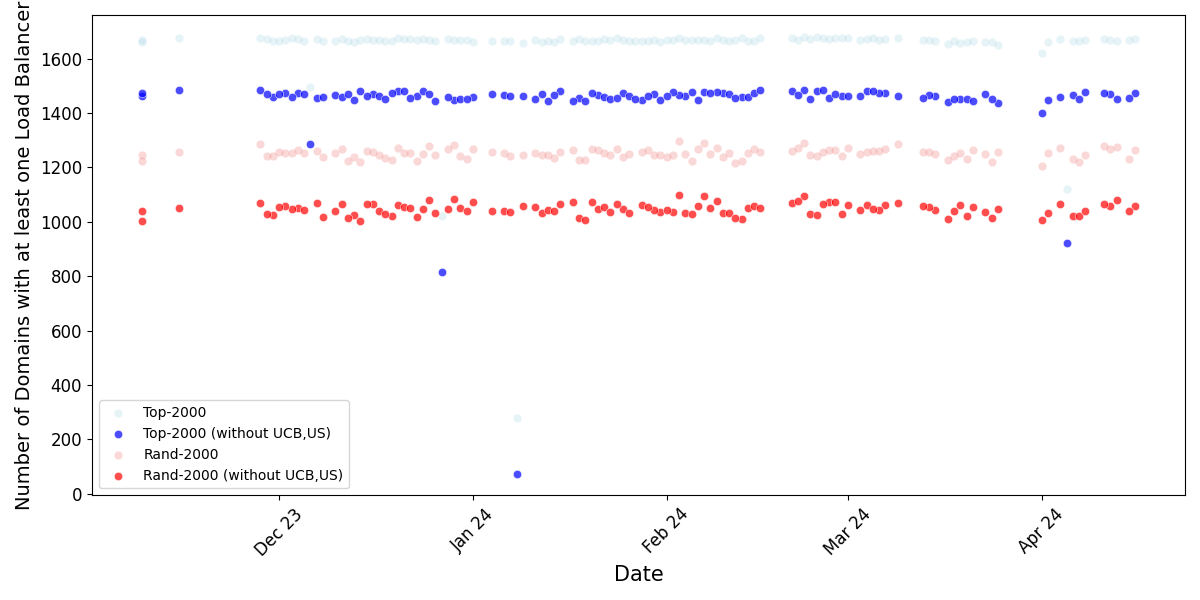
\includegraphics[width=\textwidth]{figures/scatter_plot_domains.png}
    \caption{Number of Domains with at least one Load Balancer Over Time}
    \label{fig:scatter_plot_domains}
\end{figure}
\subsection{Comparison and Insights}


The higher average and median values in the Top-2000 dataset underscore the higher usage of load balancers in managing traffic for the most visited websites. These sites likely experience higher and more variable traffic, necessitating robust load balancing solutions to ensure uptime and performance. Meanwhile, the Rand-2000 dataset demonstrates that load balancing is also very prevalent for a broad spectrum of domains.





\section{Analysis of Common Next Hops}
The analysis over a dataset from 02-21-2024 \textbf{(I will change this to include over the whole time, just wanted to give an example, won't be included in final)} revealed a total of 262 common next hops shared by at least three load balancers across different domains. The distribution of these common next hops is illustrated in Figure \ref{fig:common_next_hops_distribution}. The bar chart shows the frequency of next hops shared by varying numbers of load balancers, providing insights into the prevalence of shared network paths.

\begin{figure}[h]
    \centering
    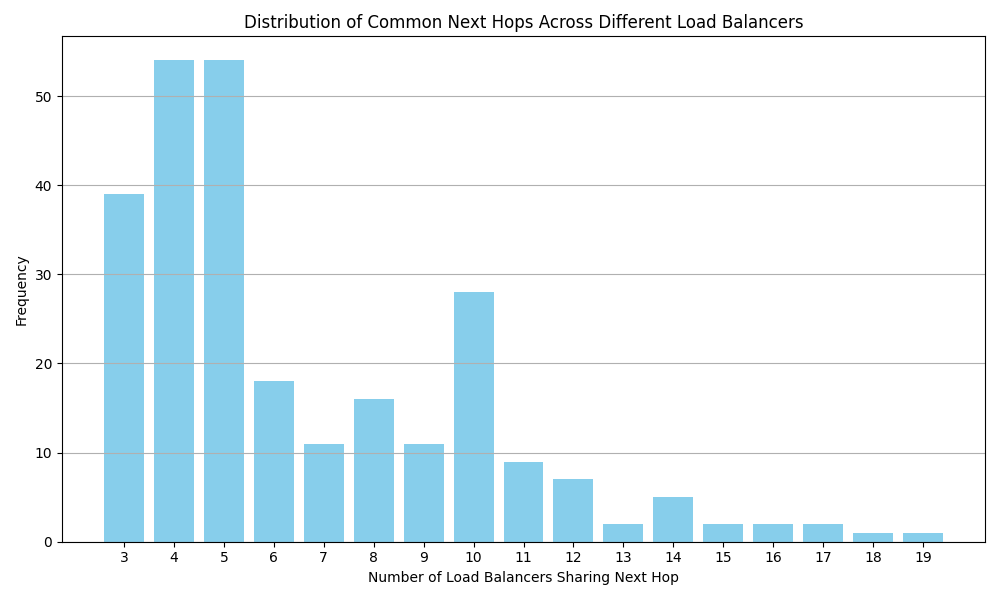
\includegraphics[width=0.8\textwidth]{figures/common_next_hops_distribution.png}
    \caption{Distribution of Common Next Hops Across Different Load Balancers }
    \label{fig:common_next_hops_distribution}
\end{figure}

With 262 occurrences of next hops shared by at least three load balancers, it suggests that network providers often deploy load balancers in a centralized manner. This results in multiple load balancers directing traffic to a common set of next hop IP addresses within the same Autonomous System (AS). This strategy likely enhances network performance and redundancy.

Another possibility is that load balancers may lead to other load balancers, creating a layered load balancing architecture. This could result in shared next hops across different domains as traffic is further distributed. These hypotheses were further tested by examining the AS information for the load balancers and their next hops, which will be detailed in the next section. Understanding these patterns is crucial for comprehending the deployment and operation of load balancers in the Internet's topology.



\chapter{This is the Sixth Chapter}
\chapter{This is the Seventh Chapter}
\chapter{This is the Eighth Chapter}


%If you have appendices to your thesis, place them here
\appendix

\chapter{Questionnaire}

\printbibliography[heading=bibintoc]

\end{document}
